\documentclass[sigconf]{acmart}

\usepackage{enumitem}
\usepackage{framed}
\usepackage[11pt]{moresize}
\usepackage{cprotect}
\usepackage{enumitem}
\usepackage{listings}
\usepackage{amstext}
\usepackage{amstext}
\usepackage{pdfpages}
\usepackage{alltt}
\usepackage{epstopdf}
\usepackage{xspace,colortbl}
\usepackage[USenglish]{babel}
\usepackage{multirow}
\usepackage{url}
\usepackage{graphicx}%%
\usepackage{amssymb}
\usepackage{fmtcount}
\usepackage{amsfonts}
\usepackage{xspace}
\usepackage{amsmath}
\usepackage{multirow}
\usepackage[mathscr]{eucal}
%\usepackage{psfrag}
\usepackage{colortbl}
\usepackage{times}


\usepackage{bm}
%\usepackage[nospace]{cite}
\usepackage{csquotes}
\usepackage{enumitem}

\lstset{basicstyle=\small,breaklines=true,language=Python,belowcaptionskip=.1\baselineskip}

\usepackage{balance}

%\linespread{0.99}

\copyrightyear{2017} 
\acmYear{2017} 
\setcopyright{acmcopyright}
\acmConference{HILDA'17}{May 14, 2017}{Chicago, IL, USA}\acmPrice{15.00}\acmDOI{http://dx.doi.org/10.1145/3077257.3077271}
\acmISBN{978-1-4503-5029-7/17/05}

\begin{document}

\setlength{\belowdisplayskip}{3pt} \setlength{\belowdisplayshortskip}{3pt}
\setlength{\abovedisplayskip}{3pt} \setlength{\abovedisplayshortskip}{3pt}
\setlength{\belowcaptionskip}{-10pt}
\selectfont

\newcommand{\cond}{\textrm{pred}\xspace}
\newcommand{\dataset}{data set\xspace}
\newcommand{\datasets}{data sets\xspace}
\newcommand{\spview}{\textsf{SPView}\xspace}
\newcommand{\fjview}{\textsf{FJView}\xspace}
\newcommand{\aggview}{\textsf{AggView}\xspace}
\newcommand{\hashfunc}[1]{\textsf{hash}(#1)\xspace}
\newcommand{\hashop}{\textsf{hash}\xspace}
\newcommand{\nsc}{\textsf{NormalizedSC}\xspace}
\newcommand{\rsc}{\textsf{RawSC}\xspace}

\newcommand{\avgfunc}{\ensuremath{\texttt{avg} }\xspace}
\newcommand{\maxfunc}{\ensuremath{\texttt{max} }\xspace}
\newcommand{\minfunc}{\ensuremath{\texttt{min} }\xspace}
\newcommand{\histfunc}{\ensuremath{\texttt{histogram\_numeric} }\xspace}
\newcommand{\countfunc}{\ensuremath{\texttt{count}}\xspace}
\newcommand{\sumfunc}{\ensuremath{\texttt{sum} }\xspace}
\newcommand{\varfunc}{\ensuremath{\texttt{var} }\xspace}
\newcommand{\stdfunc}{\ensuremath{\texttt{std} }\xspace}
\newcommand{\covfunc}{\ensuremath{\texttt{cov} }\xspace}
\newcommand{\corrfunc}{\ensuremath{\texttt{corr} }\xspace}
\newcommand{\medfunc}{\ensuremath{\texttt{median} }\xspace}
\newcommand{\percfunc}{\ensuremath{\texttt{percentile} }\xspace}
\newcommand{\havingfunc}{\ensuremath{\texttt{HAVING} }\xspace}
\newcommand{\selectfunc}{\ensuremath{\texttt{select} }\xspace}
\newcommand{\ratio}{\ensuremath{\rho }\xspace}


\newcommand{\insertion}{\ensuremath{\texttt{INSERT} }\xspace}
\newcommand{\update}{\ensuremath{\texttt{UPDATE} }\xspace}
\newcommand{\delete}{\ensuremath{\texttt{DELETE} }\xspace}

\newcommand{\sysfull}{Partition Aware Local Model\xspace}
\newcommand{\sys}{PALM\xspace}
\newcommand{\sysnospace}{PALM}

\newcommand{\tbl}[1]{\textsf{#1}\xspace}
\newcommand{\field}[1]{\textsf{#1}\xspace}
\newcommand{\cost}{\textrm{cost}\xspace}
\newcommand{\ans}{\textsf{ans}\xspace}
\newcommand{\dans}{\Delta\textsf{ans}\xspace}
\newcommand{\cqp}{correction query processing\xspace}
\newcommand{\Cqp}{Correction query processing\xspace}

\newcommand{\gray}[1]{{{\textcolor{lightgray}{\{#1\}}}\xspace}}
\newcommand{\ewu}[1]{{{\textcolor{red}{\{ewu: #1\}}}\xspace}}
\newcommand{\reminder}[1]{{{\textcolor{magenta}{\{\{\bf #1\}\}}}\xspace}}
\newcommand{\specialcell}[2][c]{%
  \begin{tabular}[#1]{@{}c@{}}#2\end{tabular}}

\def\ojoin{\setbox0=\hbox{$\bowtie$}%
  \rule[-.02ex]{.25em}{.4pt}\llap{\rule[\ht0]{.25em}{.4pt}}}
\def\leftouterjoin{\mathbin{\ojoin\mkern-5.8mu\bowtie}}
\def\rightouterjoin{\mathbin{\bowtie\mkern-5.8mu\ojoin}}
\def\fullouterjoin{\mathbin{\ojoin\mkern-5.8mu\bowtie\mkern-5.8mu\ojoin}}


\newcommand{\stitle}[1]{\vspace{0.5em}\noindent\textbf{#1}}


%\setlength{\belowcaptionskip}{-10pt}

%\newcommand{\reminder}[1] {}

%\input{coverletter.tex}

%\title{ActiveClean: Progressive Data Cleaning For Convex Data Analytics}
%\title{Towards Machine Learning Model Explanations That Are Useful For Debugging}
\title{\sys: Machine Learning Explanations For Iterative Debugging}

%\numberofauthors{2}


\author{Sanjay Krishnan}
\affiliation{{UC Berkeley}}
\email{sanjaykrishnan@berkeley.edu}

\author{Eugene Wu}
\affiliation{{Columbia University}}
\email{ewu@cs.columbia.edu}


%\fontsize{9pt}{11pt}
%\selectfont




\begin{abstract}
Emerging applications for machine learning in computer vision and natural language processing are using ever more complex and high-dimensional models.
To effectively debug such applications,  we argue that developers need a form of data provenance, namely, where they can isolate a small set of training examples that explain why a new example was predicted in a certain way.
Linking a prediction to responsible training data allows a data scientist to look for inconsistencies between training and test data, and understand the structure of a complex model.
The challenge is that in most models are coupled in nature where every training example contributes to a prediction in some way.
We present \sysfull (\sys), which approximates a complex model (e.g., a deep neural network) using a two-part surrogate model: a meta-model that partitions the training data, and a set of sub-models that approximate the patterns within each partition.
The user can use \sys to guide data exploration to identify problematic examples in the training dataset.
Queries to \sys are nearly 30x faster than nearest neighbor queries for identifying relevant data, which is a key property for interactive applications.
\end{abstract}

\maketitle

\pagenumbering{gobble}


\section{Introduction}\label{intro}

\ewu{This paragraph is misleading.  Cut it down to one sentence, combine with next paragraph.}
Systems and algoirthms for training models are so fast that it is no longer the bottleneck in the process of deploying machine learning models.
In particular, building models is not one-shot and requires iterating between model/feature design, analyzing the results, and repeat (the HILDA loop, cite last year's hilda paper).
\gray{The availability of data and vast cloud-based computational resources is allowing both industry and academia to apply Machine Learning in many new domains.
Learning-based components are increasingly in the critical path of important software systems such as in fraud detection, product recommendation, robotics and control, and machine vision.  Several breakthroughs in recent years have resulted in improved computational efficiency~\cite{feng2012towards, tensor, recht2011hogwild, crotty2014tupleware} as well as ease of development for learning applications~\cite{hellerstein2012madlib, keystone, kraska2013mlbase}.  This research has culminated in the development of several open-source toolkits with highly efficient distributed optimization libraries, e.g., TensorFlow, MLlib, and CAFFE, or in other words--training a statistical model has never been easier.}

However, surveys of data scientists, the ones who have ostensibly benefited the most from these breakthroughs, paint a very different picture~\cite{kandel2012, krishnan2016hilda}.
Building and debugging data-driven applications remains to be time-consuming and effort-intensive~\cite{sculley2014machine}.
When a prediction is unexpected, it is unclear if this is due to a data error (i.e., an inconsistent value representation), a model error (i.e., the model class cannot represent such a relationship), or an approximation error (i.e., such examples were not encountered in sufficient number during training).
When models are opaque, diagnosing such problems is difficult, so \emph{interpretability} is often touted as a solution \cite{?}.


As deeper models (DNNs) become more popular than ever, it is increasingly difficult to know what the model is learning and why the model mispredicts.
Specifically, when a prediction is unexpected, it is unclear if this is due to errors values in the training data that led to a poor model prediction, using a model  that cannot represent the patterns in the training data (e.g., need more layers?),  or an approximation error due to data simply not present in the training data.
For instance, consider designing prediction models for self driving cars.  
Poor lighting conditions, street obstacles, and other issues could lead to highly noisy training data.
Furthermore, it is unlikely that the training data has collected data for every possible driving condition (e.g., during a once in five years storm~\cite{bayareastormin2017})

In the context of DNNs, the architecture matters, however the primary source for prediction quality is a large corpus of representative training data.  
Thus, in contrast to tradiitional machine learning debugging, which seeks to idenitfy human-understandable features that most affected a given model prediction, it is more valuable to identify subsets of the training data that can help {\it explain} what most likely affected a given prediction.
\ewu{Describe why this problem is so hard that even coarse grained explanations are valuable.}
\ewu{Describe how, if your technique does work, it actually facilitates HILDA}



\ewu{I didn't believe this argument because it offers an arbitrary proposal.  Stole some of its ideas though.}
\gray{But, interpretability means different things to different people. To an end-user, this means explain why I received a given prediction in terms of understandable features. However, an ML developer cares less about understandable features than an explanation of the occurrence of an anomaly in terms of data that the model previously saw. Even if this explanation is course-grained, it is still useful as the data scientist can use this to trigger further exploratory data analysis to understand the underlying patterns. So perhaps, the models for interpretability being studied in the ML community are more complex than what we need for ML debugging.
}

Instead, we propose the admittedly imprecise notion of \emph{debugability}.
Let $M$ be a model trained on a dataset of feature and label tuples $(x_i,y_i)$.
Suppose, M sees a new example $x'$ and predicts $y'$ causing a \emph{prediction anomaly} (i.e., incorrect prediction or unsafe output).
Debugability is a measure of how well can we isolate tuples in the training dataset that significantly contributed to the prediction $y'$.

Using this working definition, we can actually design algorithms that take in a black-box model and return a more debugable approximation.
The key insight is that complex models tend to be hierarchical in nature.
One can think of a complex model as a collection of more compartmentalized models (ones that only apply to certain types of examples), and a meta model that selects which one of the sub-models is relevant to the example at hand.
In prior work, we have developed algorithms that can take a set of predictions from a model and infer a likely hierarchical structure~\cite{DBLP:journals/corr/KrishnanGLMPG16, Krishnan17}.
The basic idea is an iterative clustering algorithm that first initializes $k$ models, then assigns tuples to the model that best predicts it, then updates the $k$ models and repeats.
Once the k models are trained, we can then learn a meta-model to switch between them.
When a new example for prediction comes in, the meta-model first picks a sub-model, then the sub-model issues a prediction.
Our initial results have demonstrated that such an approach can improve convergence and stability in control problems.

This paper presents a special case of this framework aimed at improving debugging in large-scale ML settings. 
In particular, we allow the $k$ sub-models to be as expressive and complex as the user desires, but constrain the meta-model to be a decision tree.
This means that if a particular new example $x'$ creates an anomalous output, we can immediately blame a particular sub-model.
Furthermore, the decision tree allows us to quickly determine a predicate to select the subset of training data that contributed to the sub-model.
By varying $k$ and the depth of the decision tree, the user can tradeoff fidelity to the original model and the granularity of such explanations.


Our main justification is that modern ML models are necessarily complex, i.e., they often map complex data structures such as images or documents to decisions. Trying to explain every model in terms of its features, is not a tractable solution with current algorithms. Instead, if we can merely explain the high-level structure of a model (while the sub-models are still opaque), this might be enough of a signal for a data scientist to debug. As an analogy, a high-school physics teacher has to simplify the calculus in his lesson, but leaves enough detail for interested students to learn more on their own.




























\section{Framework and API}
The developer has a training dataset $D$ that consists of tuples of features $x_i$ and labels $y_i$ (either categorical or real-valued). She applies some function to this dataset $\textsf{train}(D)$, and returns a model $\textsf{model}(\cdot)$. Given a new $x_{new}$ this model returns a prediction $\hat{y}_{new}$:
\[
\hat{y}_{new} = \textsf{model}(x_{new})
\]

\vspace{0.5em}\noindent \textbf{Example Insurance Fraud Detection: } Consider the following running example of car insurance fraud detection. The training dataset $D$ has the following schema:
\[
\texttt{D(model, amount, at\_fault, description, fraud?)}
\]
where \texttt{model} is a categorical attribute describing the model of the car, \texttt{amount} is a double-valued amount that the person is claiming, \texttt{at\_fault} is a boolean variable describing whether the claimant is at fault, \texttt{description} is a string-valued attribute describing the nature of the claim, and \texttt{fraud?} is the yes/no label if the claim is fraudulent.

The function $\textsf{model}(\cdot)$ takes in a new unlabeled tuple:
\[
x_{new} = \texttt{r(model, amount, at\_fault, description, \_)}
\]
and predicts:
\[
\texttt{r(model, amount, at\_fault, description,} \hat{y}_{new} )
\]

\subsection{Challenges in Debugging}
Suppose $\textsf{model}(\cdot)$ issues an incorrect prediction and erroneously flags a fraudulent claim as not fraudulent. The data scientist is now tasked with debugging the model to understand why this error happened. 
She considers three possibilities: 
\begin{itemize}
\item \emph{(P1) Model Error.} The model is not sufficiently accurate enough to predict all claims correctly and needs to be tuned to err on the side of false positives.
\item \emph{(P2) Approximation Error.} The model was not trained with sufficient examples that look like $x_{new}$, and therefore, is not accurate in that region of the feature space.
\item \emph{(P3) Data Error.} The record $x_{new}$ is not consistent with respect to the training data, i.e., it represents the same information differently--leading to an unpredictable featurization.
\end{itemize}
The challenge for the data scientist is to determine which of these categories of errors best describes why the claim was mispredicted.
Intuitively, her process is to look at how ``similar'' tuples in the training dataset were predicted and compare to the given record. This will allow her to evaluate whether the problem is inherent to the model class or due to a fault of the training dataset or data processing pipeline. 

Existing approaches: 
\begin{itemize}
\item \emph{(S1) Nearest Neighbors. } The data scientist can search for the k nearest neighbors in the training dataset and use those as a guide.

\item \emph{(S2) Use A Simpler Model.} The data scientist can use any number of techniques to use the interpretable model from the start, then apply her domain expertise to understand why an error occurred.
\end{itemize}

The problem with (S1) and (S2) is that the models that are needed for such decision problems are necessarily complex. In the running example, there is a textual field \textsf{description}, which might be a very valuable feature for predicting fraud. Processing such data may require several NLP steps like a word-embedding, stop word removal, bi-gram featurization etc. So by design the feature space is complex and may not be interpretable by anyone other than an expert, and using a simpler model may not achieve the desired accuracy. Furthermore, as we move to a world where highly deep expressive models, which in principle can learn any deterministic function, it is well-known that these models have adversarial examples (i.e., imperceptible perturbations to the features that cause a change in prediction) \cite{szegedy2013intriguing}. This makes approaches like a nearest neighbor approach unreliable or even misleading. The approach that we propose identifies records that the classifier treats as similar, not just similarity in the feature space.

\subsection{Towards Debuggable Surrogates}
Let us consider the following working definition.
Debuggability is a measure of how well can we isolate tuples in the training dataset that significantly contributed to the prediction $ \hat{y}_{new}$.
We explore whether we given $\textsf{model}(\cdot)$ can train a surrogate model $\textsf{smodel}(\cdot)$ that approximates the original model, but is more debuggable.
One can think of a complex model as a collection of more compartmentalized models (ones that only apply to certain types of examples), and a meta model that selects which one of the sub-models is relevant to the example at hand.

This is a piecewise approximation of a complex function and by changing the allowed class models for the submodels and metamodel, we can get different behavior. 
As an illustrative example, consider when the meta model is much simpler.
For example, imagine if we hard-coded the following logic:
\begin{lstlisting}
def smodel(x):
    if amount > 10000:
    #one model for larger claims
        return submodel_1(x)
    elif a_fault:
    #one model for small at fault claims
        return submodel_2(x)
    else:
    #a default model
        return submodel_3(x)
\end{lstlisting}
Even though the logic that switches between the the submodels is simple (in fact it is a decision tree), the actual behavior is complex since the submodels encapsulate the complexity.
But, if we were to observe an anomaly, we would be able to precisely blame one of the submodels; thereby, getting a coarse predicate to select tuples that are assinged to that model.
there is an inherent tradeoff here where increasing the complexity of the meta-model improves the granularity of debugging, but potentially sacrifices on fidelity to the original model.

\subsection{Learning Meta Models} 
We propose an algorithm to automatically learn a meta-model and submodels from data to approximate the user's desired model.
This algorithm can run offline during the training phase and is generally no-more than a constant factor more expensive than standard model training
This algorithm is a special case of the algorithm, we proposed in prior work~\cite{DBLP:journals/corr/KrishnanGLMPG16, krishnan17}. At a high-level, the algorithm takes the dataset $D$ and the model \textsf{model} as input, and returns $\textsf{smodel}$, which consists of a decision-tree meta model that selects from a collection of $k$ submodels. Given a new record, the user can evaluate both:
\[
\hat{y}_{new} = \textsf{model}(x_{new})
\]
\[
\hat{y}_{new} = \textsf{smodel}(x_{new}) \approx \textsf{model}(x_{new})
\]
and use the structure of \textsf{smodel} to debug with knowledge that it approximates $\textsf{model}$.

\subsection{API and System}
We implemented this as a system in Python initially focusing on TensorFlow models.
For the user, the inputs are:
\begin{itemize}
\item \emph{Featurized Dataset. } The user provides a dataset of feature and label tuples.

\item \emph{Explainable Features. } The user lists a subset of features that are understandable.

\item \emph{Tensorflow Model Description. } The user provides a symbolic description of the model in Tensorflow.

\item \emph{Number of Sub-models. } The user provides the number of submodels to include in the surrogate model (denoted as $k$).
\end{itemize}

The output of the system is:
\begin{itemize}
\item \emph{Original Model. } The original model trained to completion

\item \emph{K Sub-Models. } The system returns K submodels trained on different partitions of the feature-space.

\item \emph{Decision Tree Meta Model. } The system returns a meta model that switches between the K submodels based on the input record.
\end{itemize}

We implemented the algorithm into a web interface that allows users to debug TensorFlow models Figure \ref{fig:interface}. The interface shows users mispredictions and allows them to search records that the classifier treats as similar.

\begin{figure*}[t]
    \centering
    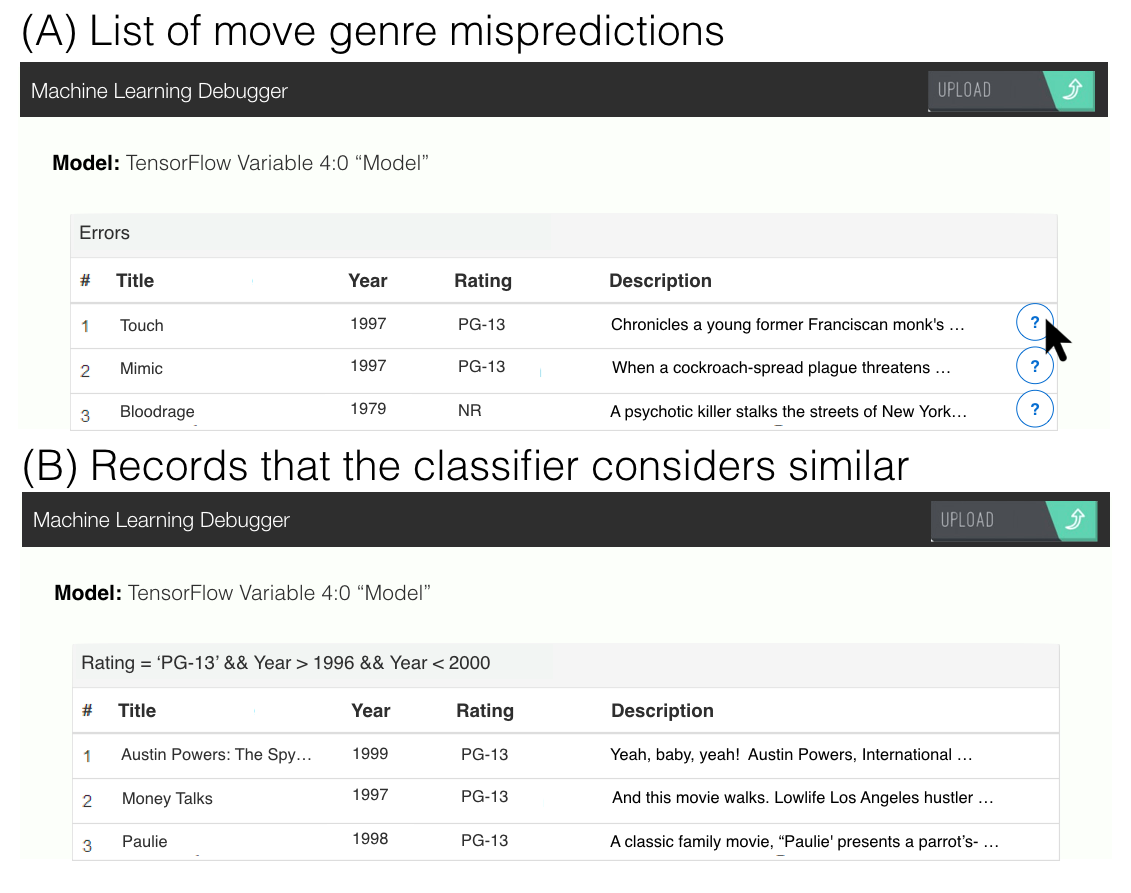
\includegraphics[width=0.6\textwidth]{figures/interface.png}
    \caption{A prototype interface implementing the algorithm. In (A), the interface lists a set tuples that were mis-predicted. Users can dig deeper by selecting one such tuple. (B) is the following panel which describes a predicate and records that the classifier considers as similar.}
    \label{fig:interface}
\end{figure*}
\section{Algorithm Description}
In prior work, we designed an algorithm in a completely different context---to decompose complex control policies to reduce planning horizons~\cite{DBLP:journals/corr/KrishnanGLMPG16, Krishnan17}. Surprisingly, when we started discussing our ideas with ML developers, we realized a very similar approach could apply for problems in debugging. 

For intuition on how the algorithm works, consider a standard KMeans clustering of dataset. First, $k$ random cluster centers are placed over the feature-space. Then, data are assigned to the nearest cluster. Finally, the clusters are updated based on the assignment, and the algorithm repeats by re-assigning data based on the most recent update.

Similarly, we can do the same thing for model training. $k$ random sub-models are initialized.
During the ``assignment'' step, a data point is assigned to the sub-model that best predicts it.
Then, during the update step, the models are updated based on the new assignments with gradient descent.
This is a variant of the popular Expectation-Maximization algorithm, that instead of a Maximization step, computes a gradient instead. 

This algorithm to run efficiently at scale and directly integrate with TensorFlow's Python API.
So, at training time (offline) the user can not only train the original model but also the surrogate.
We also integrated the algorithm into a local web interface that visualized the results.


\subsection{Technical Details}

\vspace{0.5em} \noindent \textbf{Fitting Step: } To construct $\textsf{smodel}(\cdot)$ from $\textsf{model}(\cdot)$, we first start off by fitting the parameters to a simplified probabilistic model. 
The first step is to run $\textsf{model}(\cdot)$ over the entire training dataset and get feature-prediction $(x, \hat{y})$ tuples.
We can define $f(\hat{y} \mid x)$ which is the probability of the label $\hat{y}$ given the feature $x$ to represent how $\textsf{model}(\cdot)$ generates predictions. 
Arbitrary probability distributions are hard to reason about so we consider parametrized distributions $f(\hat{y} \mid x, \theta)$. 
We want to find $k$ such distributions that best explain all the observations:
\[
\{f(\hat{y} \mid x, \theta_1),...,f(\hat{y} \mid x, \theta_k)\}
\]
Our results in prior work~\cite{?,Krishnan17} show how this can be optimized with a two-step algorithm:
\begin{itemize}
    \item Initialize $\theta_1,...,\theta_k$ randomly.
    \item Repeat until convergence
    \item For each data point $i \in \{1,...,N\}$: 
    \item \begin{itemize} 
          \item For each component distribution $j \in \{1,...,k\}$:
          \item $w(i,j) = f(\hat{y}_i \mid x_i, \theta_j)$
    \end{itemize}
    \item Gradient Ascent for each $\theta$:
    \[ \theta_j \leftarrow \theta_j + \lambda \sum_i^N w(i,j) \nabla \log f(\hat{y}_i \mid x_i, \theta_j)  \]
\end{itemize}

The intuition behind this algorithm is that after random initialization the initial models will have higher accuracy on different data points (by chance). $w(i,j)$ is a soft-assignment--assigning data points to the model that best explains its prediction. Then, $w(i,j)$ becomes a weight to update the models with Gradient Ascent (or descent over the negative log likelihood). This, process repeats until convergence. This is very similar to the K-Means or EM algorithm but instead of updating the cluster centers with a formula, we take a gradient step.

\vspace{0.5em} \noindent \textbf{Distillation Step: } The result of the first step is a set of model parameters $k$ $\theta_1,...,\theta_k$, and a weighting function $w(i,j)$. The next step is to distill $w(i,j)$ into a set of explainable rules that select the one of the $k$ models. We first generate a set of hard assignments for each data point:
\[
h(i) = \arg\max_{j} w(i,j)
\]
Each $h$ is an indicator $1,...,k$ of the most likely assignment of each data point.
We can now train a more explainable model to select $h$ as a function of the data.
This intuition is that this is a simpler model that just selects one of the component models.

The user provides us with a list of features that are considered ``explainable'', and let $x_e$ denote the projection of an example onto this subset of features.
Then, we can train a Decision Tree over the tuples $(x_e, h)$, which have the desirable property of resembling programatic statements.
We call this model the meta-model, as it selects between the component models.

Finally, putting everything together, we return something that looks similar to the hard-coded example in the previous section:
\begin{lstlisting}
def smodel(x):
    if amount > 10000:
        return f_theta1(x)
    elif a_fault:
        return f_theta2(x)
    else:
        return f_theta3(x)
\end{lstlisting}
The surrogate model $\textsf{smodel}(\cdot)$ encapsulates submodels that apply in different parts of the feature-space.
Suppose, we observe an anomaly, we can now blame a specific model and efficiently get a predicate that selects all of the data the contributed to the model.
\input{interface.tex}

\iffalse
\begin{figure*}[ht]
    \centering
    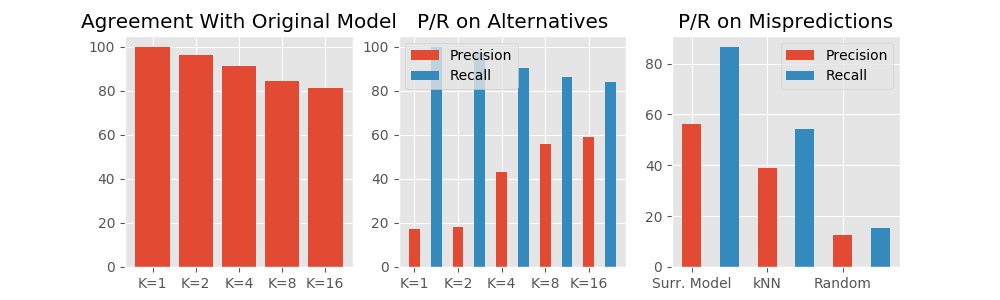
\includegraphics[width=\textwidth]{figures/result1.png}
    \caption{(A) Illustrates how a \sys  model can approximate a complex model, (B) illustrates how well this surrogate model can isolate mispredictions in terms of precision and recall, and (C) why alternative approaches do not work.}
    \label{fig:teaser}
\end{figure*}
\fi

\section{Highlighted Experiments}
This section presents key experimental results that highlight use cases where \sys models can help identify training data that cause mispredictions, 
when \sys diverges from the user's more complex model, and a comparison with alternative explanation approaches. 

\subsection{Setup}
We consider the following scenario. Suppose, the model receives a previously unseen test point that is mispredicted, can we identify the subset of training data that ``influences'' this prediction error. 
\sys returns a subset of training data using the hierarchical approximation, but we could, in principle, apply the following approaches to select relevant training data: 

\vspace{0.25em} \noindent \textbf{Nearest Neighbors: } Suppose, we measure influence purely in terms of similarity to the new data point. We could select the k-nearest neighbors in the training dataset and return them to the user. We set $k$ to be the same as number of data points returned by \sys for the new data point.

\vspace{0.25em} \noindent \textbf{Clustering: }
Another approach would be to cluster the training examples, and then return the cluster closest to the new data point. We use K-Means and set the number of clusters to 10. 

\vspace{0.25em} \noindent \textbf{Random: } Finally, as a baseline, we could randomly select training examples.  We set the number of selected examples to be the same as number of data points returned by \sys for the new data point.

\noindent \vspace{0.5em} We measure influence in the following way.
If a sample of labels of the training data outside of the selected subset are randomly perturbed, and the model is retrained, how often does the prediction change. In other words, this is a measure how ``true'' the selected neighborhood is w.r.t how the model implicitly partitions the feature space.

\subsubsection{Datasets}
We split each dataset into a training dataset $80\%$ and test dataset $20\%$. 
\stitle{Movie: } We have a dataset of movie descriptions IMDB~\footnote{ \url{ftp://ftp.fu-berlin.de/pub/misc/movies/database/}} and Yahoo~\footnote{ \url{http://webscope.sandbox.yahoo.com/catalog.php?datatype=r}}.
Each movie has a title, a short 1-2 paragraph plot description, year, rating, language, and a list of categories, and the goal is to train a model to predict whether a movie is a ``Horror'' or ``Comedy'' from the description and title.  
The total dataset has 506,244 records.
First, using TensorFlow, we trained a LSTM-based model to predict these categories. The first layer of this model computes what is called a word-embedding, where the LSTM learns a feature-space in which similar words (co-occuring) are closer together. 
The next two layers consist of dense layers that map the words from the feature-space to classification outputs.
The result is a model that achieves 93\% accuracy, which is far more accurate than simpler alternatives on a Bag-of-Words featurization (random forests 90\%, Linear SVM 81\%, Kernel SVM 85\%).

\stitle{Fraud: } ProPublica collected a dataset of corporate donations to medical researchers to analyze conflicts of interest~\cite{dollarsfordocs}. 
Records contain the PI's medical specialty, the drug brand name (null if not drug), the device brand name (null if not a device), name of pharamceutical donor, the amount donated, and whether the research is disputed.
The dataset comes with a \texttt{status} field that describes whether or not the donation was allowed under the declared research protocol.
We used a Multi-Layer Perceptron to classify disallowed donations which achieved a 82\% accuracy (random forest 81\%, Linear SVM 80\%, Kernel SVM 80\%).

\subsection{Experiments}

\stitle{Exp 1. Isolating Mispredictions } 
In the first experiment, we illustrate one benefit of \sys in terms of how it can explain predictions in terms of subsets of training data. We measure the quality of an explanation in the following way: (1) select a test data point that is mispredicted, (2) construct an explanation of this prediction by selecting a subset of training data, (3) for all examples outside of the selected subset randomly flip the labels of 25\% of the points, (4) retrain the model and observe if the test data point changes its prediction. 
We run 1000 trials of this procedure for 10 randomly sampled mispredictions and plot the results in Figure \ref{fig:isolation}. 
This metric measures how well isolated the selected neighborhood is from the other points--in other words, if the other points were changed how much would the prediction change.
The random baseline changes it prediction roughly 25\% of the time.
The clustering and the nearest neighbor approaches only consider the feature-space, not the structure of the classifier.
While they are significantly more robust than random (< 5\%) prediction changes, \sys is much more robust (< 1 \%) prediction changes.

\begin{figure}[ht]
    \centering
    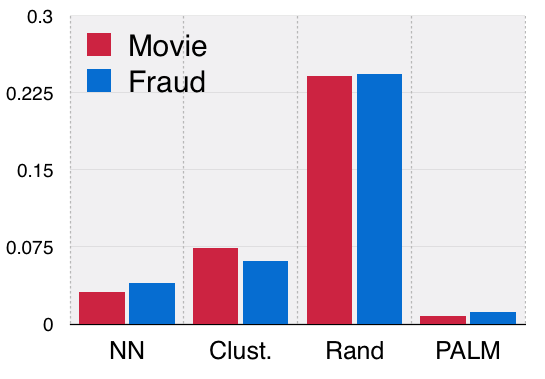
\includegraphics[width=0.7\columnwidth]{figures/isolation.png}
    \caption{\sys isolates relevant training data more effectively than baselines.}
    \label{fig:isolation}
\end{figure}

\stitle{Exp 2. Discovering other Misprediction with \sys }  
In the next experiment, we explore whether mispredictions concentrate around particular submodels. We train the models on 80\% of the dataset, and test on the remaining 20\%. We measure the fraction of mispredictions attributed to each submodel. We want to show that mispredictions concentrate around specific submodels and are not evenly distributed throughout the feature-space. Figure \ref{fig:concentrate} shows this effect when we apply our algorithm to approximate the Movie and Fraud models with $k=10$ submodels. For the Movie dataset, 70\% of the mis-predictions are attributed to a single submodel.
For the Fraud dataset, 78\% of the errors are attributed to two of the submodels.

\begin{figure}[ht]
    \centering
    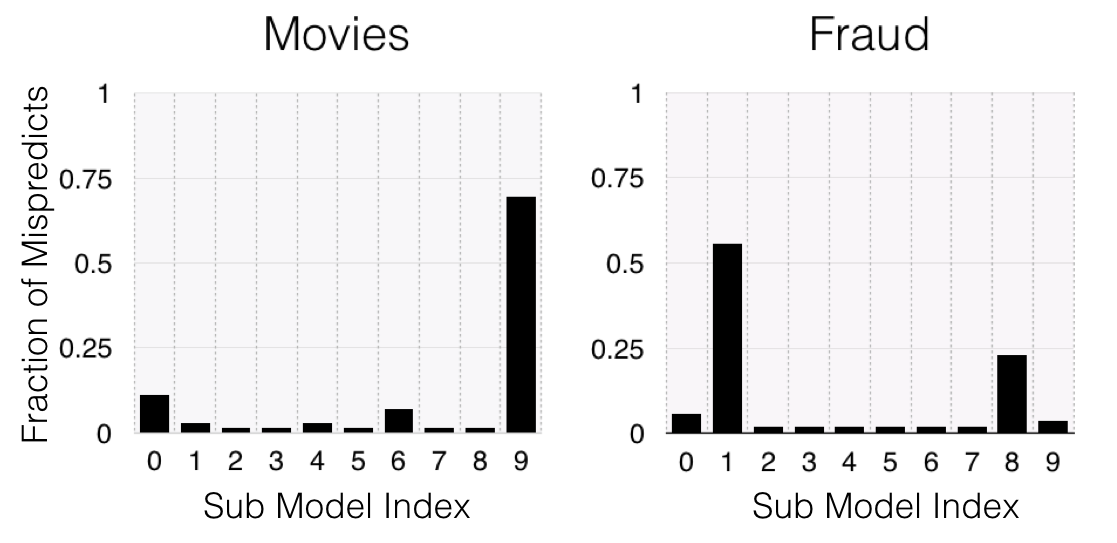
\includegraphics[width=\columnwidth]{figures/concentration.png}
    \caption{On two datasets, we show how mispredictions concentrate around specific submodels. This means there are specific regions of the feature-space most associated with mispredictions.}
    \label{fig:concentrate}
\end{figure}

\stitle{Exp 3. Agreement With the Original Model}
We now measure the agreement between the \sys model with the original model as we increasing the number of partitions $k$ (Figure~\ref{fig:agreement}, where agreement is the accuracy with respect to the original model.
We find that with $k=16$, both \sys models still retain $>90\%$ agreement with the original model.
This suggests that \sys can help developers identify more precise subsets of the training data while still trusting that the \sys models are reflective of the original model.

\begin{figure}[ht]
    \centering
    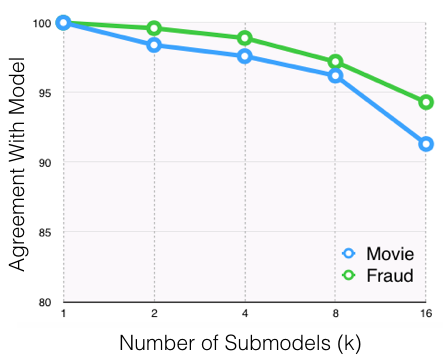
\includegraphics[width=0.6\columnwidth]{figures/agreement.png}
    \caption{On two datasets, we find that the discretized models agree with greater than 90\% accuracy with the original model. As the number of submodels increase the accuracy goes down.}
    \label{fig:agreement}
\end{figure}


\stitle{Exp 4. \sys is efficient} 
\sys can run offline during training time and queries to \sys are very efficient as it simply involves a decision tree evaluation.
\sys is explicitly designed to mimic the user's model, and the decision tree learned by the meta-model can easily be used to index or partition the training data can be indexed.
For the nearest neighbors approach, it is possible to quickly find the neighbors by using intelligent indexing structures such as KD-trees or Oct-trees.  However spatial indices are well known to have difficulty scaling to very high dimensional datasets.  In addition, finding the neighbors in a high dimensional space may simply not identify relevant results. One could apply dimensionality reduction but this would further reduce its efficacy.
On the other hand the clustering approach is much faster because it only requires querying each cluster center.
Our interesting insight is that \sys is much faster than the nearest neighbor approach, and competitive with the clustering approach in terms of run time.
Our approach returns more than 30x faster than a nearest neighbor search even when coupled with dimensionality reduction and a KD-Tree.
The clustering approach is much faster but \sys is still within the latencies needed for interactive latencies.

\begin{table}[ht!]
\centering
\caption{Run times of the different algorithms in seconds}
\label{my-label}
\begin{tabular}{lll}
Algorithm & Movie & Fraud \\ \hline
kNN & 35.61 & 22.11  \\
kNN+PCA & 12.34 & 6.97  \\
\sys & 0.334 & 0.31  \\
Clustering & 0.07 & 0.06
\end{tabular}
\end{table}

\section{Conclusion}
We presented \sysfull (\sys), a system to explain a model's prediction in terms of relevant training data.  \sys decomposes a complex model (e.g., a deep neural network) using a two-part {\it surrogate model}: a meta-model that partitions the training data, and a set of sub-models that approximate the patterns within each partition.
These sub-models can be arbitrarily complex to capture local patterns. However the meta-model is constrained to be a decision tree.
This formulation ensures that sub-models are accurate, while the partitions are interpretable as rules.
In contrast to existing model interpretation techniques that return locally relevant features, our approach returns the most informative neighborhood (partition).
Our experiments show that we can generate Fast And Clear Explanations using \sys.
We show that the explanations found by \sys select subsets of data that better align with the structure of the original model than the nearest neighbor or clustering baseline.
Furthermore, we show that \sys is nearly 30x faster than a nearest neighbor query, which is the next most accurate baseline.
\section{Related Work}
The study of model intepretability and explainability is recently a hot topic in ML research~\cite{taylor2016alignment, lei2016rationalizing, ribeiro2016should}, especially in the context of Neural Networks. 

%\input{problem_statement.tex}
%\input{architecture.tex}
%\input{naive.tex}
%\input{detector.tex}
%\input{sampling.tex}
%\input{estimator.tex}
%\input{optimal.tex}
% \input{detect.tex}

% \input{impestimate.tex}

%\input{optimizer.tex}
%\input{experiments.tex}
%\section{Related Work}
The study of model intepretability and explainability is recently a hot topic in ML research~\cite{taylor2016alignment, lei2016rationalizing, ribeiro2016should}, especially in the context of Neural Networks. 
%\input{discussion.tex}
%\input{conclusion.tex}
%\input{outlier.tex}
%\input{analysis.tex}
%\input{experiments.tex}
%\input{conclusion.tex}


%\bibliographystyle{abbrv}
%\scriptsize

\vspace{0.5em}
\noindent \textbf{Acknowledgements: }
This research was supported in part by a seed grant from the UC Berkeley Center for Information Technology in the Interest of Society (CITRIS), the UC Berkeley RISELab, and by the U.S. National Science Foundation under Award IIS-1227536: Multilateral Manipulation by Human-Robot Collaborative Systems. This work has been supported in part by funding from Google and and Cisco.


%\fontsize{8.8pt}{9.9pt} \selectfont
\bibliographystyle{ACM-Reference-Format}
\bibliography{ref,explainability} 
\normalsize \selectfont
%\appendix
%\input{appendix.tex}

\end{document}
